\noindent Here we finish study of the quantum Klein-Gordon field by working out how the Lorentz group is unitarily represented on the space of states on the Klein-Gordon field. Recall that for a relativistic quantum field theory, we must have a (projective) unitary representation of the Poincar\'e group $U(\Lambda, a)$ on a Hilbert space $\mathcal{H}$. Thus far, we have constructed the Hilbert space, with respect to some norm $|| \cdot ||$, as the space of states gotten by applying creation operators to the vacuum state

\begin{equation}
\mathcal{H} = span \{ \hat{a}_{\textbf{p}_1}^\dagger \hat{a}_{\textbf{p}_2}^\dagger \dots \hat{a}_{\textbf{p}_n}^\dagger \ket{\Omega} \} ^{||\cdot||}
\end{equation}

\subsection*{Digression: Continuous Groups of Symmetries}

\noindent The central idea of a group with a continuous manifold structure (e.g., Lie groups) is to study symmetries close to, localized to, the identity and then exponentiate to larger, more global, elements. Important continuous operations on this manifold $\mathcal{M}$ include (closed) composition and inverse. \\

\begin{figure}[H]
	\centering
	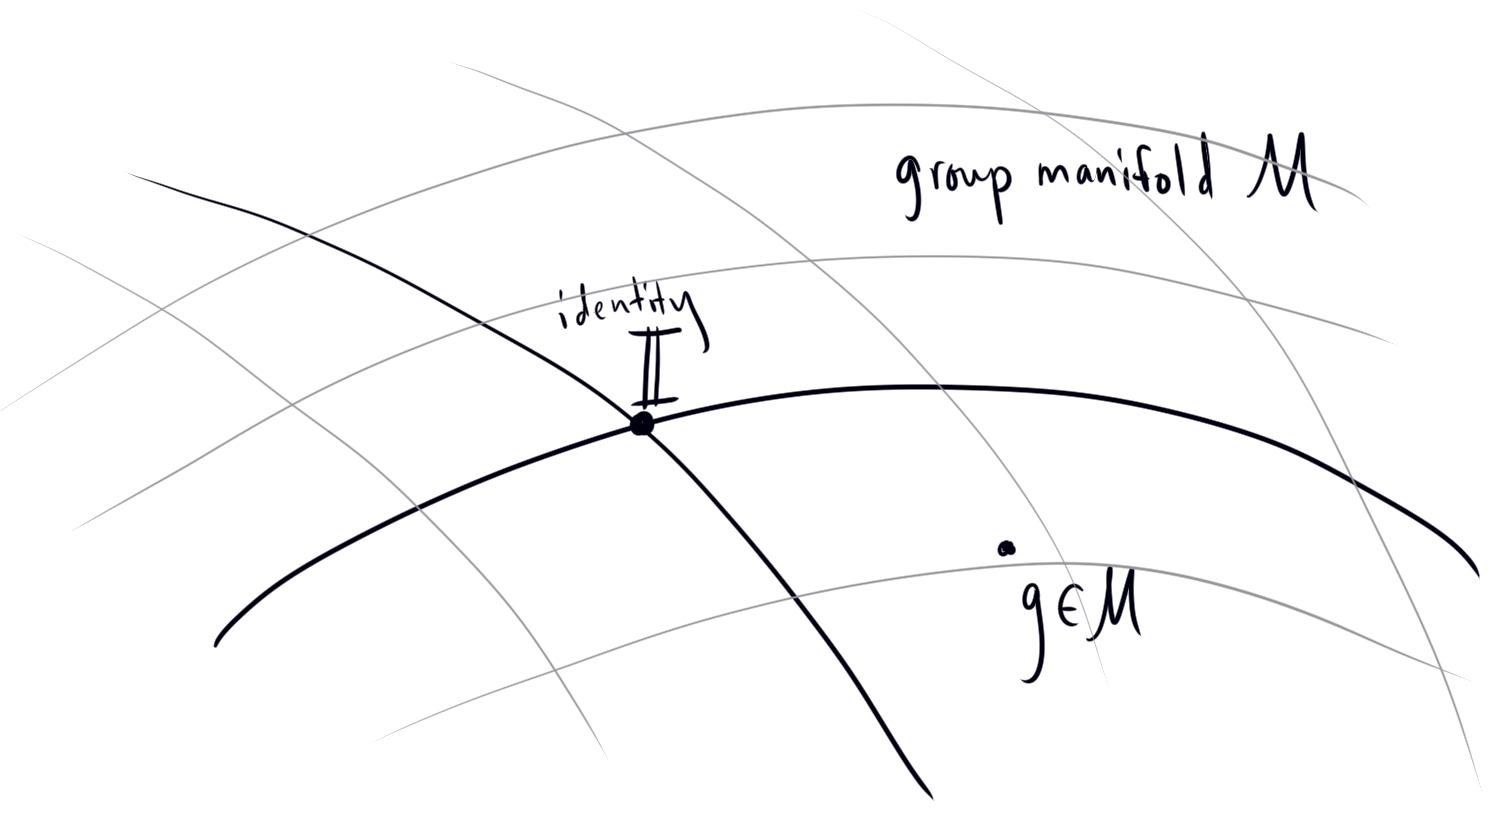
\includegraphics[scale=0.3]{images/groupmanifold.png}
	\caption{Sketch of a group manifold with identity $\mathbb{I}$ and an element of the manifold $g$.}
\end{figure}

\begin{align}
\text{Closure:} \,\,\,\,\, \mathcal{M} \times \mathcal{M} &\rightarrow \mathcal{M} \\
g \times h &\rightarrow g \cdot h \\
\text{Inverse:} \,\,\,\,\,\,\,\,\,\,\,\,\,\,\,\,\,\,\,\, \mathcal{M} &\rightarrow \mathcal{M} \\
g &\rightarrow g^{-1}
\end{align}

\noindent The Poincar\'e group is an example of a continuous Lie group, and to understand its structure, consider elements $g \in \mathcal{M}$ infinitesimally close to the identity $\mathbb{I}$, such that $g - \mathbb{I} \sim \mathcal{O}(\epsilon)$. These infinitesimal elements are elements of the tangent space $T_{\mathbb{I}} \, \mathcal{M}$, which is a linear space and is called a \textit{Lie algebra}. The basis vectors of $T_{\mathbb{I}} \, \mathcal{M}$ are written as $x^j$, $j=1,2,\dots,dim(\mathcal{M})$.

\subsection*{Examples of Tangent Spaces}

\begin{enumerate}
\item $1 \times 1$ unitary matrices $U(1) = \{ \phi \in \mathbb{C} : |\phi|^2 = 1 \}$
\subitem $\rightarrow T_1 \, U(1) = \{ z: (1+\epsilon z)^* (1+\epsilon z) = 1$ to order $\epsilon$,  s.t. $Re[z]=0) \}$

\item $3 \times 3$ Euclidean rotation matrices $O(3) = \{ O \in \mathcal{M}_3(\mathbb{R}) : O^T O = \mathbb{I} \}$
\subitem $\rightarrow T_{\mathbb{I}} \, O(3) = \{ X : (\mathbb{I} + \epsilon X)^T (\mathbb{I} + \epsilon X) = \mathbb{I}$ to order $\epsilon$, s.t. $X + X^T = 0 \}$
\subitem - Note that including inversions promotes $O(3)$ to $SO(3)$.
\subitem - Basis of $O(3) = \\ \{ X = \sum_{j=1}^3 X_j J^j : J^1 = \left(\begin{smallmatrix} 0&1&0 \\ -1&0&0 \\ 0&0&0 \end{smallmatrix}\right), J^2 = \left(\begin{smallmatrix} 0&0&1 \\ 0&0&0 \\ -1&0&0 \end{smallmatrix}\right), J^3 = \left(\begin{smallmatrix} 0&0&0 \\ 0&0&1 \\ 0&-1&0 \end{smallmatrix}\right) \}$

\item $4 \times 4$ Lorentz transformation matrices $G = \{ \Lambda : \eta_{\mu\nu} \Lambda^\mu_{\,\,\,\rho} \Lambda^\nu_{\,\,\,\sigma} = \eta_{\rho\sigma} \}$ 
\subitem \begin{align*}
\rightarrow T_{\mathbb{I}} \, G &= \{ \omega : \eta_{\mu\nu} (\mathbb{I} + \epsilon \omega)^\mu_{\,\,\,\rho} (\mathbb{I} + \epsilon \omega)^\nu_{\,\,\,\sigma} = \eta_{\rho\sigma} \} \\
&= \{ \omega : \text{antisymmetric, s.t. } \omega^{\mu\nu} = -\omega^{\nu\mu} \} \\
&\,\,\,\,\,\,\, {\scriptsize \text{Note the "upstairs" covariant indices on }} \omega \\
&\,\,\,\,\,\,\, {\scriptsize \text{Using "downstairs" contravariant indices}} \\ 
&\,\,\,\,\,\,\, {\scriptsize \text{requires multiplication by the metric } \eta_{\mu\nu} \text{ as above.}} \\
&= \{ \omega : \text{change of basis to } \omega = \sum_{j=1}^6 \frac{1}{2} \Omega_j J^j \} \\
&\,\,\,\,\,\,\, {\scriptsize \text{Change indices via the bijection } j \rightarrow (\rho \, \sigma), \text{with } 0<\rho<\sigma\le 3 } \\
&\,\,\,\,\,\,\,\,\,\,\,\,\,\,\,\,\,\, 1 \rightarrow (0 \, 1); \, 2 \rightarrow (0 \, 2); \, 3 \rightarrow (0 \, 3) \\
&\,\,\,\,\,\,\,\,\,\,\,\,\,\,\,\,\,\, 4 \rightarrow (1 \, 2); \, 5 \rightarrow (1 \, 3); \, 6 \rightarrow (2 \, 3) \\
&= \tag{\textbf{Exercise}} \{ \omega : \text{with index bijection } \omega = \sum_{(\rho\sigma)} \frac{1}{2} \Omega_{(\rho\sigma)}  J^{(\rho\sigma)}  \} \\
&\,\,\,\,\,\,\,\,\,\,\, {\scriptsize \text{This bijection allows the basis to be expressed }}  \\
&\,\,\,\,\,\,\,\,\,\,\, {\scriptsize \text{by the formula } [J^{(\rho\sigma)}]^\mu_{\,\,\nu} = \eta^{\rho\sigma} \delta^{\sigma}_{\,\,\nu} - \eta^{\sigma\mu} \delta^{\rho}_{\,\,\nu}} \\
\end{align*}
\end{enumerate}

\noindent Understanding the structure of a linear space infinitesimally close to the identity yields information about the whole Lie group and the global structure of the manifold. Also note that multiplication on this linear space is a continuous map that strongly determines the group structure on the manifold. \\

\noindent To demonstrate how a Lie algebra on the (linear) tangent space produces a Lie group, and vice versa, consider the element of the tangent space of a manifold $X \in T_{\mathbb{I}} \, \mathcal{M}$, such that $\mathbb{I} + s X \sim e^{\epsilon X} \in \mathcal{M}$, to order $\epsilon$. \\

\noindent Define the function $g(s) = \lim_{n\to\infty} (\mathbb{I} + \frac{s}{n} X)^n = e^{s X} \in \mathcal{M}$. Therefore, every element of the Lie algebra (tangent space to the identity) determines an element of the Lie group (manifold). To go the other way, and determine the Lie algebra from the Lie group, apply the logarithm map.\\

\begin{figure}[H]
	\centering
	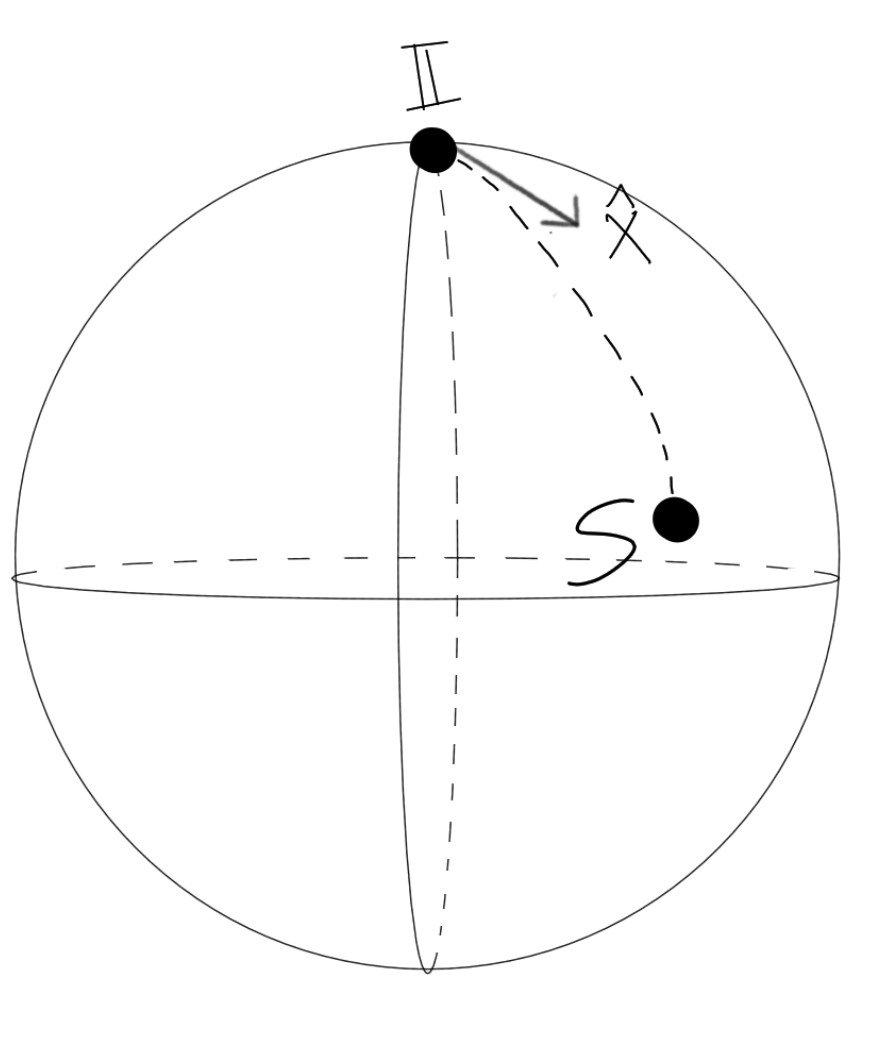
\includegraphics[scale=0.4]{images/exponentiation.png}
	\caption{Figure of exponentiation map on Lie group (e.g., $O(3)$) manifold. Translation from identity a distance $s$ along the $X$ direction. Resulting position on manifold is called the exponential of $s X$.}
\end{figure}

\subsection*{Algebraic structure on tangent space}

\noindent The algebraic structure on the tangent space is defined by the \textit{group commutator} on the manifold, which is also a group. 
\begin{align}
[\, , \,] : \mathcal{M} \times \mathcal{M} &\rightarrow \mathcal{M} \\
(g, h) &\rightarrow [g, h] = ghg^{-1}h^{-1}, \, \forall \, g, h \in \mathcal{M}
\end{align}

\noindent The group commutator also pushes forward to a mapping of the tangent space
\begin{equation}
[\, , \,] : T_{\mathbb{I}} \, \mathcal{M} \times T_{\mathbb{I}} \, \mathcal{M} \rightarrow T_{\mathbb{I}} \, \mathcal{M}
\end{equation}

\noindent Consider the following group commutator which is an element of the manifold
\begin{align}
[\mathbb{I} + \epsilon X, \mathbb{I} + \delta Y] &= (\mathbb{I} + \epsilon X) (\mathbb{I} + \delta Y) (\mathbb{I} - \epsilon X) (\mathbb{I} - \delta Y) \\
&= \mathbb{I} + \epsilon \delta (XY - YX) + \mathcal{O}(\epsilon^2) + \mathcal{O}(\delta^2) + \dots \\
&\sim \mathbb{I} + \epsilon \delta [X, Y]
\end{align}

\noindent Where $\epsilon$ and $\delta$ are small, independent parameters, and the Lie algebra commutator $[X, Y]$ is, therefore, an element of the tangent space of the manifold, such that $[X,Y] \in T_{\mathbb{I}} \, \mathcal{M}$. \\

\subsection*{Examples of Lie algebra commutators}

\begin{enumerate}
\item $U(1)$: trivial
\item $O(3)$: $[J^j, J^k] = -\epsilon^{jk}_{\,\,\, l} J^l$ 
\item Lorentz group: $[J^{\rho\sigma}, J^{\tau\nu}] = \eta^{\sigma\tau}J^{\rho\nu} - \eta^{\rho\tau}J^{\sigma\nu} + \eta^{\rho\nu}J^{\sigma\tau} - \eta^{\sigma\nu}J^{\rho\tau}$

\subitem E.g., \[ [J^{01}]^\mu_{\,\,\, \nu} = 
\left( 
\begin{array}{@{}c|c@{}}
\begin{matrix} 0 & 1 \\ 1 & 0 \end{matrix} & \bigzero \\
\hline
\bigzero & \begin{matrix} 0 & 0 \\ 0 & 0 \end{matrix} 
\end{array} \right), \,\, [J^{12}]^\mu_{\,\,\, \nu} = 
\left( 
\begin{array}{@{}c|c@{}}
\bigzero & \begin{matrix} 0 & 0 \\ -1 & 0 \end{matrix} \\
\hline
\begin{matrix} 0 & 1 \\ 0 & 0 \end{matrix} & \bigzero
\end{array} \right) \]

\subitem \[ [J^{01}, J^{12}] = -J^{13} =  
\left( 
\begin{array}{@{}c|c@{}}
\bigzero & \begin{matrix} 0 & 0 \\ 0 & -1 \end{matrix} \\
\hline
\begin{matrix} 0 & 0 \\ 0 & 1 \end{matrix} & \bigzero
\end{array} \right) \]

\subitem Special names for this particular Lie group elements in the Lorentz transformation
\subsubitem \textbf{Generators of boosts} (pure boost by exponentiating, s.t. $e^{\frac{1}{2} \epsilon_j K^j}$): 
\subsubitem $J^{0j} = K^j$
\subsubitem \textbf{Generators of rotations} (elements of $O(3) \subset$ Lorentz group): 
\subsubitem $J^{12} = J^1, \, J^{13} = J^2, \, J^{23} = J^3$
\end{enumerate}

\subsection*{Representations of Lie groups}

Consider a representation $\pi$ of the Lie algebra $T_\mathbb{I}\,\mathcal{M}$ which is a linear map from the tangent space to the Hilbert space of bounded linear operators, such that the Lie bracket property is preserved, such that $[\pi(X), \pi(Y)] = \pi([X,Y])$
\begin{equation}
\pi : T_\mathbb{I}\,\mathcal{M} \rightarrow \mathcal{B} (\mathcal{H})
\end{equation}

\noindent This representation is exponentiated to a representation of the Lie group manifold $\mathcal{M}$
\begin{equation}
\pi(g = e^{\epsilon X}) = e^{\epsilon \pi(X)}
\end{equation}

\noindent This shows that one can either try to find matrices that obey the Lie group law, or, more easily, focus on the Lie algebra (linear space) and find matrices that obey the Lie bracket property; Lie group representations are often not worked with directly, but the elements of the Lie algebra can just be exponentiated to obtain the representation of the Lie group. \\

\noindent To implement a general Lorentz transformation on the Hilbert space of states allowed in the Klein-Gordon field, Noether's theorem, as well as the \textit{inverse Noether's theorem}, is employed. Noether's theorem allows conserved currents to be derived from symmetry transformations. Information in thrown out when integrating the currents over space $\int d^3 x$ to get the conserved charge, but the time-like component is left alone, and information about the structure of the symmetry transformation is conserved, which can be gotten back by the inverse Noether's theorem. \\

\noindent \textbf{Recap of Noether's theorem:} For each symmetry of a field, with respect to a coordinate transformation $x \rightarrow \exp^{\epsilon J ^{\rho\sigma}}$, there exists a conserved current per $J^{\rho\sigma}$. For example, the group of Lorentz transformations is described by six independent parameters, the generators of the transformation, associated with six conserved currents. The conserved currents from the symmetries of the Lorentz transformation have the form
\begin{equation}
\mathcal{J}^{(\rho\sigma)} = \textbf{x}^\rho T^{\mu\sigma} - \textbf{x}^\sigma T^{\mu\rho}
\end{equation}

\noindent Where $\textbf{x}^\mu$ are 4-vector spacetime coordinates, and $T^{\mu\nu}$ are elements of the energy-momentum tensor. The conserved charges are then gotten by integrating over space
\begin{equation}
Q^{(\rho\sigma)} = \int d^3 x \, \mathcal{J}^{(\rho\sigma)} = \int d^3x \,  (\textbf{x}^\rho T^{0\sigma} - \textbf{x}^\sigma T^{0\rho})
\end{equation}
\\
\textit{"Noether's theorem is really just a fancy telescoping series in disguise."} \\

\noindent The arguably more profound statement regarding conserved charges and symmetries is the inverse Noether's theorem. \\

\noindent \textbf{Inverse Noether's theorem:} Conserved charges are the generators, represent the Lie algebra, of the symmetry transformations from which they came, and generate canonical transformations, or representations of the symmetries, on phase space. Classically, 
\begin{equation}
\{Q^{(\rho\sigma)}, Q^{(\tau\nu)}\}_{PB} = \eta^{\sigma\tau}Q^{\rho\nu} - \eta^{\rho\tau}Q^{\sigma\nu} + \eta^{\rho\nu}Q^{\sigma\tau} - \eta^{\sigma\nu}Q^{\rho\tau}
\end{equation}

\noindent Propose that we "just put hats on" the conserved charges, and check that they obey the Lie algebra of the Lorentz group. It turns out that this works for free theories, and we have, at least, one representation of the Lie algebra of the Lorentz group in the context of one, the Klein-Gordon, quantum field.
\begin{equation}
\hat{Q}^{\mu\nu} = \int d^3 x (x^\mu \hat{T}^{0\nu} - x^\nu \hat{T}^{0\mu})
\end{equation}

\noindent Consider the $0j^{th}$ conserved charge, using the specialized notation, and check that $\hat{Q}^{0j} = \hat{K}^j$ does indeed generate boosts and is time independent.
\begin{align}
\hat{Q}^{0j} = \hat{K}^j &= \int d^3 x \, (x^j \hat{T}^{00} - x^0 \hat{T}^{0j}) \\
\hat{K}^j &= -t \, \hat{P}^j + \int d^3 x \, x^j \hat{\mathscr{H}}(t,x) \\
\frac{d \hat{K}^j }{dt} &= -\hat{P}^j + i [\hat{H}, \int d^3 x \, x^j \hat{\mathscr{H}}(t,x) ] \\
0 &= \hat{P}^j + i[\hat{H}, \hat{K}^j] \\
[\hat{H}, \hat{K}^j] &= -i \hat{P}^j .
\end{align}

\noindent Where $\hat{P}^j$ is the total field momentum, and $\hat{\mathscr{H}}$ is the Hamiltonian density, which does not commute with the Hamiltonian $\hat{H}$. The third line cancels the time dependence of the two right-hand side terms. This shows that an infinitesimal shift in time and an infinitesimal boost is equal to an infinitesimal shift in space. \\

\noindent Similarly for the generators of rotation, which are manifestly time independent, it must be checked that they obey the correct Lie algebra. 
\begin{equation}
\hat{J}^{jk} = \int d^3 x \, \hat{\pi}(x)(x^j \partial_k - x^k \partial_j) \hat{\phi}(x)
\end{equation}

\noindent To perform a Lorentz transformation on the Hilbert state space, a unitary operator is created by putting some parameters $\Omega$ in front of the generators of rotation and exponentiating
\begin{equation}
\hat{U}(\Lambda) = e^{-\frac{1}{2} \Omega_{\rho\sigma} \hat{J}^{\rho\sigma}}
\end{equation}

\noindent There are 9 commutation relations, that must be checked (\textbf{Exercises}), that yield the full Lie algebra of the Poincar\'e group.
\begin{align}
[\hat{J}^j, \hat{J}^k] &= -i \epsilon^{jk}_{\,\,\,\,l} \hat{J}^l \\
[\hat{J}^j, \hat{K}^k] &= -i \epsilon^{jk}_{\,\,\,\,l} \hat{K}^l \\
[\hat{K}^j, \hat{K}^k] &= i \epsilon^{jk}_{\,\,\,\,l} \hat{J}^l \\
[\hat{J}^j, \hat{P}^k] &= -i \epsilon^{jk}_{\,\,\,\,l} \hat{P}^l \\
[\hat{K}^j, \hat{P}^k] &= i \delta^{jk} \hat{H} \\
[\hat{K}^j, \hat{H}] &= i \hat{P}^j \\
[\hat{J}^j, \hat{H}] &=  [\hat{P}^j, \hat{H}] = [\hat{P}^j, \hat{P}^k] = 0
\end{align}

\noindent This now demonstrates how the Klein-Gordon field gives a full (Lie algebra) representation of the Poincar\'e group, and  proves that to perform a Poincar\'e transformation on a state of Klein-Gordon particles, one simply applies a unitary transformation via exponentiation of the above operators, which are the generators of transformations.